From HW~\ref{hw:mass}.\ref{chap:transfer_function_models}, the transfer function for the mass spring damper is 
\begin{equation}\label{eq:hw_mass_bode_tf}
P(s) = \frac{1/m}{s(s+b/m)} = \frac{0.2}{s(s+0.1)}.
\end{equation}
In Bode canonical form we have
\[
P(j\omega) = \frac{2}{(j\omega)(1+j\frac{\omega}{0.1})}
\]

Therefore
\[
20\log_{10}\abs{P(j\omega)}=
	20\log_{10} 2 
	-20\log_{10}\abs{j\omega}
	-20\log_{10}\abs{1+j\frac{\omega}{0.1}}.
\]
Therefore, the Bode plot for magnitude will be the graphical addition of a constant gain, an integrator, and a pole.
Similarly, the phase is given by
\[
\angle P(j\omega) = 
	\angle 2 
	- \angle (j\omega)
	- \angle (1+j\frac{\omega}{0.1}).
\]
The straight line approximation as well as the Bode plot generated by Matlab are shown in Figure~\ref{fig:hw_mass_bode}.
\begin{figure}[H]
   \centering
   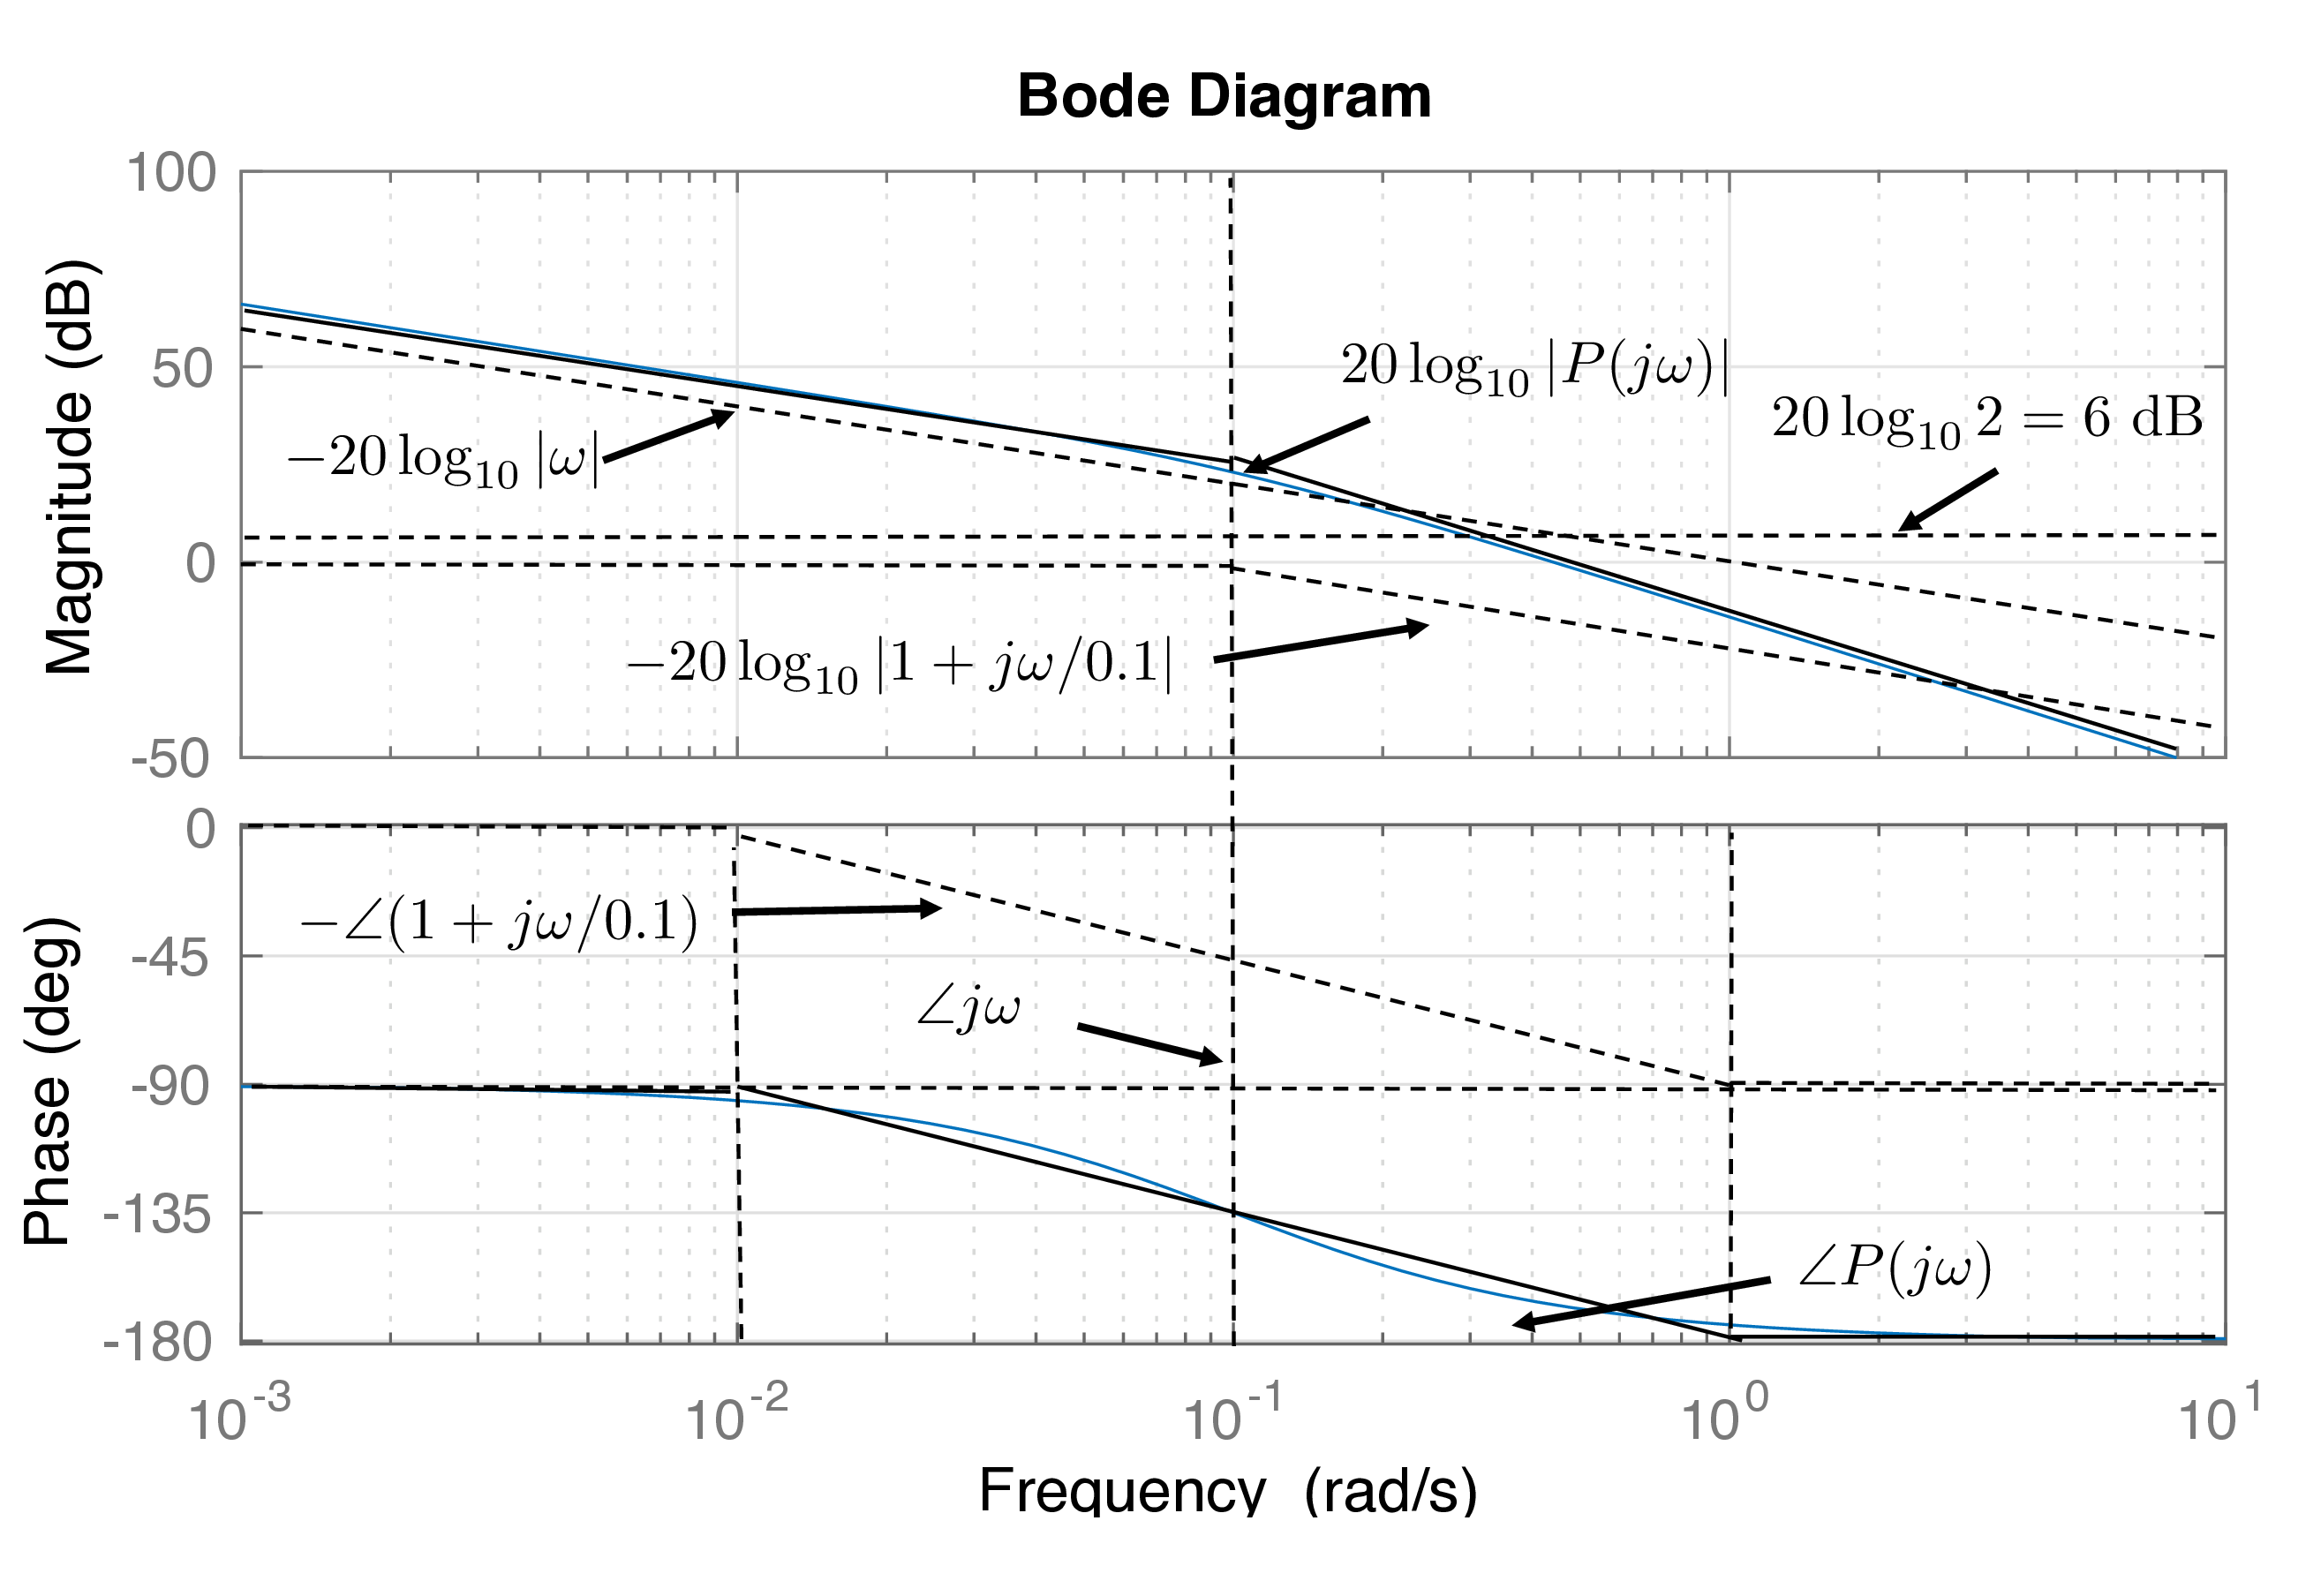
\includegraphics[width=0.9\textwidth]{6_design_studies/figures/hw_mass_bode.pdf}
   \caption{Bode plot for the transfer function given in Equation~\eqref{eq:hw_mass_bode_tf}.}
   \label{fig:hw_mass_bode}
\end{figure}

The Python command to generate the Bode plot is
\begin{lstlisting}
>> import matplotlib.pyplot as plt
>> import control as cnt
>> P = tf([.2],[1, 0.1, 0]);
>> plt.figure(1), clf, cnt.bode_plot(P), grid on
\end{lstlisting}
